\subsection{Data Description}
In order for the middleware and storage layer to make decisions
that are appropriate given the user's intentions, data must be
described in a way that communicates these intentions to
the system. In this project, we label the smallest unit of data
saved in the storage system as a \textit{chunk}.  A chunk consists of not only
raw data, but also metadata that expresses additional
knowledge about that data.
A user space variable, such as \textit{temperature}, may
consist of a collection of chunks, possibly with different accuracy or
resolution, and with each chunk representing
a different portion of the variable.
A key advantage of having attributes at this lowest level is that it allows data
semantics, user intentions, QoS requirements, and the relationship between user
data to be readily captured and embedded with the raw data so that these
smallest pieces can each be managed independently or collectively, depending on
the need. As an example, retrieving 3D field data generated from a simulation
and then visualizing it requires the coordinates and connectivity variables be
accessed simultaneously and with low latency to achieve a good user experience.
Managing data at this low level
bridges the semantics gap between applications, middleware, and storage
systems and allows the system to understand user-level data, execute QoS
requirements and policies, and optimize application and system performance.

%The new APIs will enable the bridge by specifying selectable
%performance/quality/- cost tradeoffs from both the application and system
%perspectives based upon the user guided rules/policy and runtime system
%monitoring status. It allows the middleware to make best possible decisions
%from the feedback of storage system knowledge, such that it will embed user
%intentions and the available system storage.  We want the system to give the
%users a certain amount of currency in terms of bandwidth, storage space on
%each level, and latency expectations. These notions will be fuzzy but they
%will allow the user to make ad-hoc decisions to figure out what needs to be
%saved.

The data description may be stored with the individual chunks or within a
separate metadata service or both to aid QoS requirements. It would contain
conventional attributes such as data type, size, dimensionality, and the
relationship to other data. In particular, the relationship to other chunks can
be captured by including \textit{typed links} each representing a different
relationship type.  In this project, a key metric stored as a metadata
attribute is \textit{data utility}.  It enables QoS scheduling, data placement
decisions, data lifetime decisions, and captures the chunk priority. It is
our belief that exascale science will require users to prioritize a small set
of chunks to be saved on higher-level capacity-limited storage to avoid the
slow access to large-capacity lower-level storage, such as tape.  We propose a
new technique, described by a utility function provided by a user, where chunks
can be cast into multiple data buckets and each bucket can be prioritized
differently according to its utility value.  Once this is done, the middleware
system will construct the data description and re-organize and place data to
achieve the desired QoS goals and policies.

A key insight in this proposed project has been the increased interaction of
the application with the storage system.
The user would like to have the ability to obtain information about, and even
negotiate with the system to determin what
level of Quality of Service is possible given
a prospective set of I/O operations and current state of the system, so that
they can then make decisions about what data to access when.
%for example is less than what they desire and will then place in a certain set
%of rules which the system can make autonomic decisions to help decide what
%should be done.
Towards this end, we propose to
address the QoS requirements by providing the application with mechanisms to
specify the quality of I/O service, interrogate the storage system, and react
to the responses. Guided by our past work we propose to explore the design of
mechanisms for this purpose. 

Our research will address the following questions:
1) How can users interact with the storage system efficiently?
2) How can users express their intentions into actionable items which can take place in the middleware and/or storage layer?
3) How can users annotate data with a utility metric?

\paragraph{State of the art:}
Our current data annotation techniques demonstrated in
ADIOS~\cite{lofstead:2009:adaptible} implement a binary-packed data format that
allows data characteristics such as min, max and index to be wrapped around
data chunks. A direct benefit is that each data chunk can be operated upon
independently and I/O concurrency can be maximized. We will build upon this
capability and further augment the format to express data utility.
Recently
DAMSEL~\cite{damsel} has provided a rich metadata representation and management
layer that captures the relationship between data blocks for scientific
applications.  This allows application data to be mapped to storage system
efficiently, without overburdening users with the management of complex data models, such
as AMR, from the user space. Despite these efforts, the aspect of data importance has yet to be 
explored, and we believe it will be vital for exascale storage solutions.
{\color{red}\bf there must be other work in this area, and we need to get more
references}

\paragraph{Proposed research approach:} 
We will design and develop new techniques for data management, description,
and access that allow users to describe the data utility based on their
expectations. This can be done by allowing users to plug in functions that
provide data-specific functionality to the middleware and storage system.
These functions may be executed by the system to
calculate the utility value for each chunk, handle custom compression
and decompression, and perform other data-specific services, thus allowing
the system to more effectively manage data placement and retrieval.
%
%We will design an updated I/O API that will expand on the current POSIX I/O
%semantics by adding new information to the I/O request.

We will explore the space of application level hints that can be provided easily
to the storage system. These hints will enable the storage system to make the
most appropriate optimization decisions for this user in the context of the
multi-user environment rather than trying to rely on a one-size-fits-all
approach. In particular, we expect the application to provide hints on the
length of time before the output data is persistent and visible to users and
the expected data lifetime for output sets. For read calls we envision
hints that provide latency and precision requirements. Additional hints will
also be investigated. 

We will also develop a new type of querying system that allows an application
to ask the storage system about completion timing information. The response
would be an estimated time for the described operation. We will explore
how these query functions can be integrated into common applications with
minimal code disruptions and the set of policies that applications can use to
respond to this new information. We will also explore how applications can
query the storage system to gain insights on available space in different tiers
and how applications can tailor their output data to most effectively use the available space.
Finally we will study the use of an external data annotation system that can
provide information to the storage system without requiring the application to
be recompiled. 

%
From an application level, we will explore these techniques through our ADIOS
framework using many of the applications to which we have access, including
XGC1, GTC, and SPECFM3D. We will investigate: 1) what hints the users can give
the system, 2) how the users can replace much of their
application specific code with
``system level code'' through the use of these hints.  We will design an API
that will be integrated with the storage layer to give time estimations so that
users can decide which data priorities will be written and read. The utility
value for each chunk will be used to sort the chunks into prioritized bins.
Chunks in a particular bin will be assigned an appropriate storage
 tier and lifetime, which can be decided by the user through the API.
For example: in Figure~\ref{fig:ssio-bucket} we have data that
comes from the XGC1 code.  The user can pick a data-refactoring scheme (see
Sec~\ref{sec:data-refactor}) which will bucket the particle data into 4
prioritization levels.  The user can then pick a data utility, such as 3 months
for the highest priority items and 12 months for the lowest priority data.
The user will then call a function, provided by the API, that allows them
to specify all of the chunks they want
written (particles, two fields, and a mesh in this example) and the system
will return an estimate of the time it will take to write. The user can then
use another call which will determine the lowest priority element (in this
case the user will write all of the data (P1-P4). The data will then be stored
across the layers of the file system where the two highest priority buckets
will be stored in the Parallel File System, but the next highest priority items
will be stored lower in the storage stack. 
%


\begin{wrapfigure}{r}{0.7\textwidth}
%\vspace{0ex}
        \begin{centering} 
	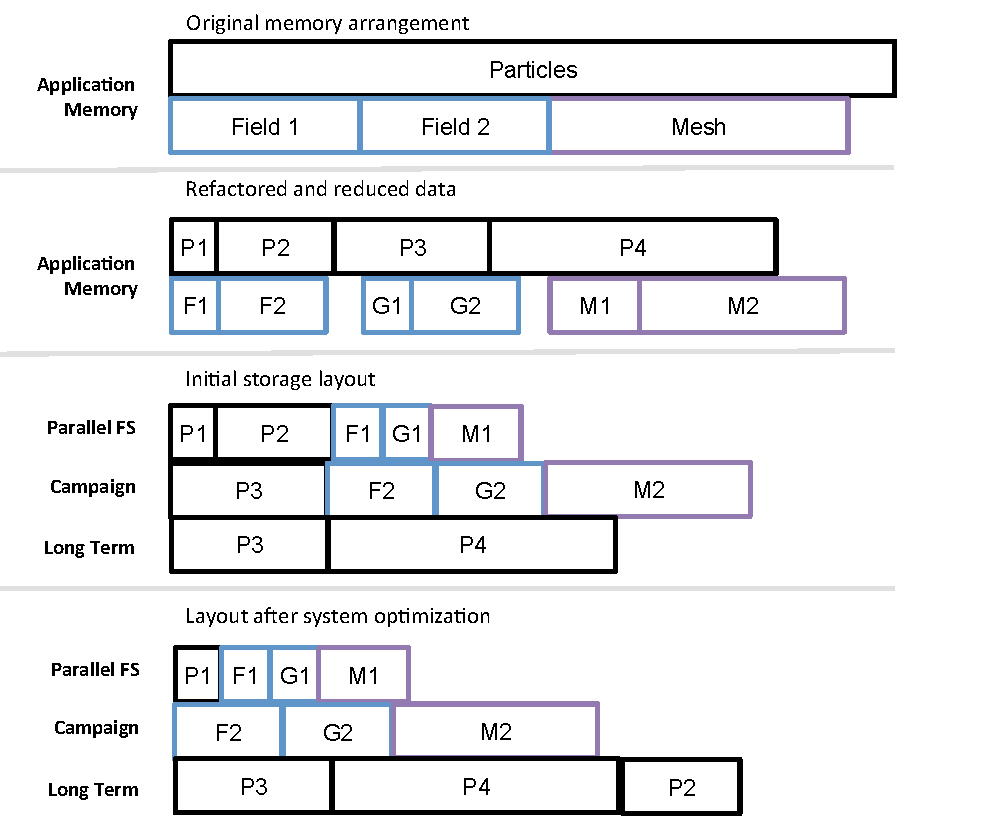
\includegraphics[scale=0.75]{graphics/SSIO-bucket.pdf}
        %\vspace{1ex}
        \caption{The system manages the data across the various stages of the data lifecycle}
        \label{fig:ssio-bucket}
        \end{centering}
%        \vspace{1ex}
\end{wrapfigure}


We will design new techniques, available to both users and the storage system,
to raise or lower these sub-chunks up and
down the storage stack. The SSIO layer will then manage the system metadata so
that the user can transparently access any of these sub-chunks without
the need to know where the data currently resides.
This requires that when reading the data, the middleware will
provide a time estimate of reading, and then allow the users to decide if
they will read less (e.g., only the highest priority sub-chunks)
if the time estimate
for reading exceeds their expectations. Existing Sirocco functionality may be
sufficient for these purposes, but it must still be proven in practice.
%

Users will also need to describe information about the data in order to choose
the optimal data-refactoring routine. Currently, we understand that
users can tell us that the data represents: 1) phase-space (e.g., the particles
in our example), 2) spatial-changes (e.g., the mesh), 3) space-time (e.g.,
the fields on the mesh). We need this information to select
the best possible data
refactoring methods. Although users can insert a user-defined data-refactoring
method, system-level methods can also use this information to make better decisions.
We will investigate new techniques and new semantics capable of using
this information to best prioritize and re-organize data.

Finally we will investigate the use of additional information
on top of the data model.
This information will be used to indicate data associations that exceed
traditional data models. For example, the fields and mesh in our example have
an inherent relationship. A common data model will describe all of the
variables in the mesh (the coordinates, the units, and the types of elements if
this were a finite-element mesh). We will explore new mechanisms that will
group data together making it explicit that M1, F1, and G1 need to be organized
together.  In other words, it will not be helpful if data from M1 and M2 were
organized together along with only F1. When the users wants to visualize data
from the field, F1, they will need only M1 and M2 would be additional
information. Likewise, if the user wants to see F1 and F2, then they will need
the mesh from M1 and M2. This requires that the time to access all of this
data is approximately the same requiring similar access times for all of the
data.  We will investigate what choices the SSIO system must make in order to
keep these pieces ``together'', from a performance perspective. Can the storage
system move everything to a lower layer when all of it doesn't fit or is there
other, less tightly related data can be evicted to preserve the collective
retrieval performance?  We need to investigate the potential problems when this
occurs and how the users can specify additional information to ensure they get
the best possible data from the SSIO layer.

We seek to provide dynamic runtime information to the user and make the
system more transparent. This would allow the end user to analyze or
visualize data in a more
predictable way since they would have more confidence of how much time
the data retrieval process would take.

%Firstly, we will explore the augmentation of I/O application programing
%interfaces (I/O APIs) to allow applications to both specify timing and quality
%information and also query the storage system for timing estimates. If user
%decide to write or read data to or from hierarchical storage systems, they
%will rely on the API to send their intentions for inquiry and examine the
%system status, including how much data they would like to write/read, desired
%bandwidth, data compression method, etc, or the user can express their
%intension of writing data right now no matter what the traffic is now.
%Through this interface we expect the application and user to gain insights
%into how long a single output or input call will take given the required
%quality information, and then react to these estimates by adjusting the
%quality or restricting the scope of the data required. Likewise we will
%explore how an application can provide timing information to the storage
%system to allow the storage system to make optimization decisions to best meet
%the requirements from the application. 
%
%Secondly, we will also explore external data annotations, such as those
%provided by the configuration file in ADIOS. Through the use of these external
%augmentation the user can provide insights to the storage system on the
%relative value of the data, expected life time and performance
%characteristics, as well as relationships between different data sets. With
%this information the storage system can make optimizations specific to a use
%case. We expect these augmentations to be particularly important for eviction
%of data from a storage layer, and migration of data sets to a different
%storage layer. 

\paragraph{Challenges:}
These new techniques offer both technical and adoption challenges. We will only
consider the technical challenges. The proposed techniques and features aim to
expose broad system level environmental information to the application and
allow the application to adapt dynamically based on this information.  One
aspect of this challenge is the design of an interrogative API that offers a
negotiation between the application and the storage system to make adaptation
decisions.  Since we will work closely with many of the leading LCF
applications, we need to make sure that our additional APIs and semantics in
the storage layer will be accepted by these applications and eventually by the
rest of the community. This requires careful examination of the full range
of possible
design choices to ensure stable APIs and useful semantics.


